\documentclass[border=10pt]{standalone}
\usepackage{pgfplots}
\pgfplotsset{compat=1.18}

\begin{document}
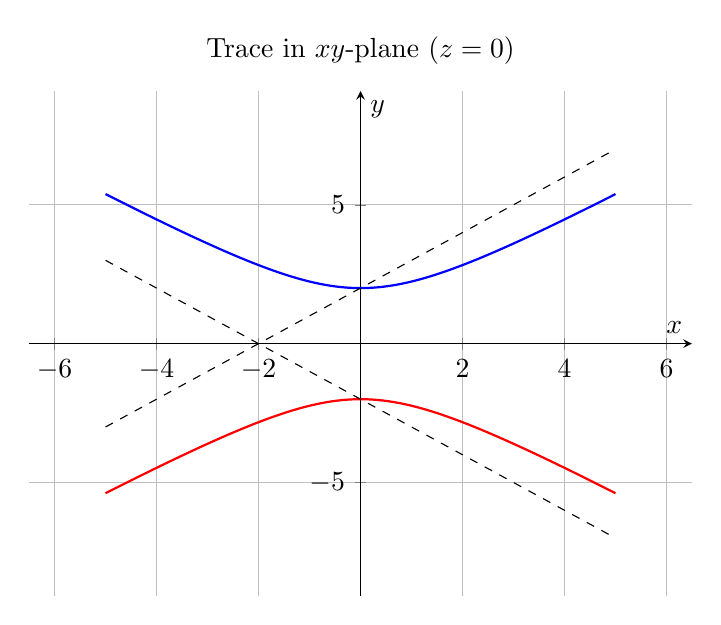
\begin{tikzpicture}
\begin{axis}[
    xlabel={$x$},
    ylabel={$y$},
    title={Trace in $xy$-plane ($z=0$)},
    width=10cm,
    height=8cm,
    axis lines=center,
    enlargelimits=0.15,
    grid=major,
    domain=-5:5,
    samples=100,
]
% Upper branch: y = 2*sqrt(1 + x^2/4)
\addplot[blue, thick] {2*sqrt(1 + x^2/4)};
% Lower branch: y = -2*sqrt(1 + x^2/4)
\addplot[red, thick] {-2*sqrt(1 + x^2/4)};
% Asymptotes
\addplot[black, dashed] {2 + x};
\addplot[black, dashed] {-2 - x};
\end{axis}
\end{tikzpicture}
\end{document}